\section{Experimental setup Calibration}

\subsection{Set-up}
\label{sec:calibration:set-up}
Before performing the source spectra measurements, the detector was connected to the HV power supply and to an amplifying circuit consisting of a \textit{preamplifier} and a \textit{coarse-gain amplifier}, shown on respectively in figure \ref{fig:preamp_photo} and \ref{fig:ampli_gene}. 

\begin{figure}[H]
  \begin{subfigure}[b]{0.45\textwidth}
    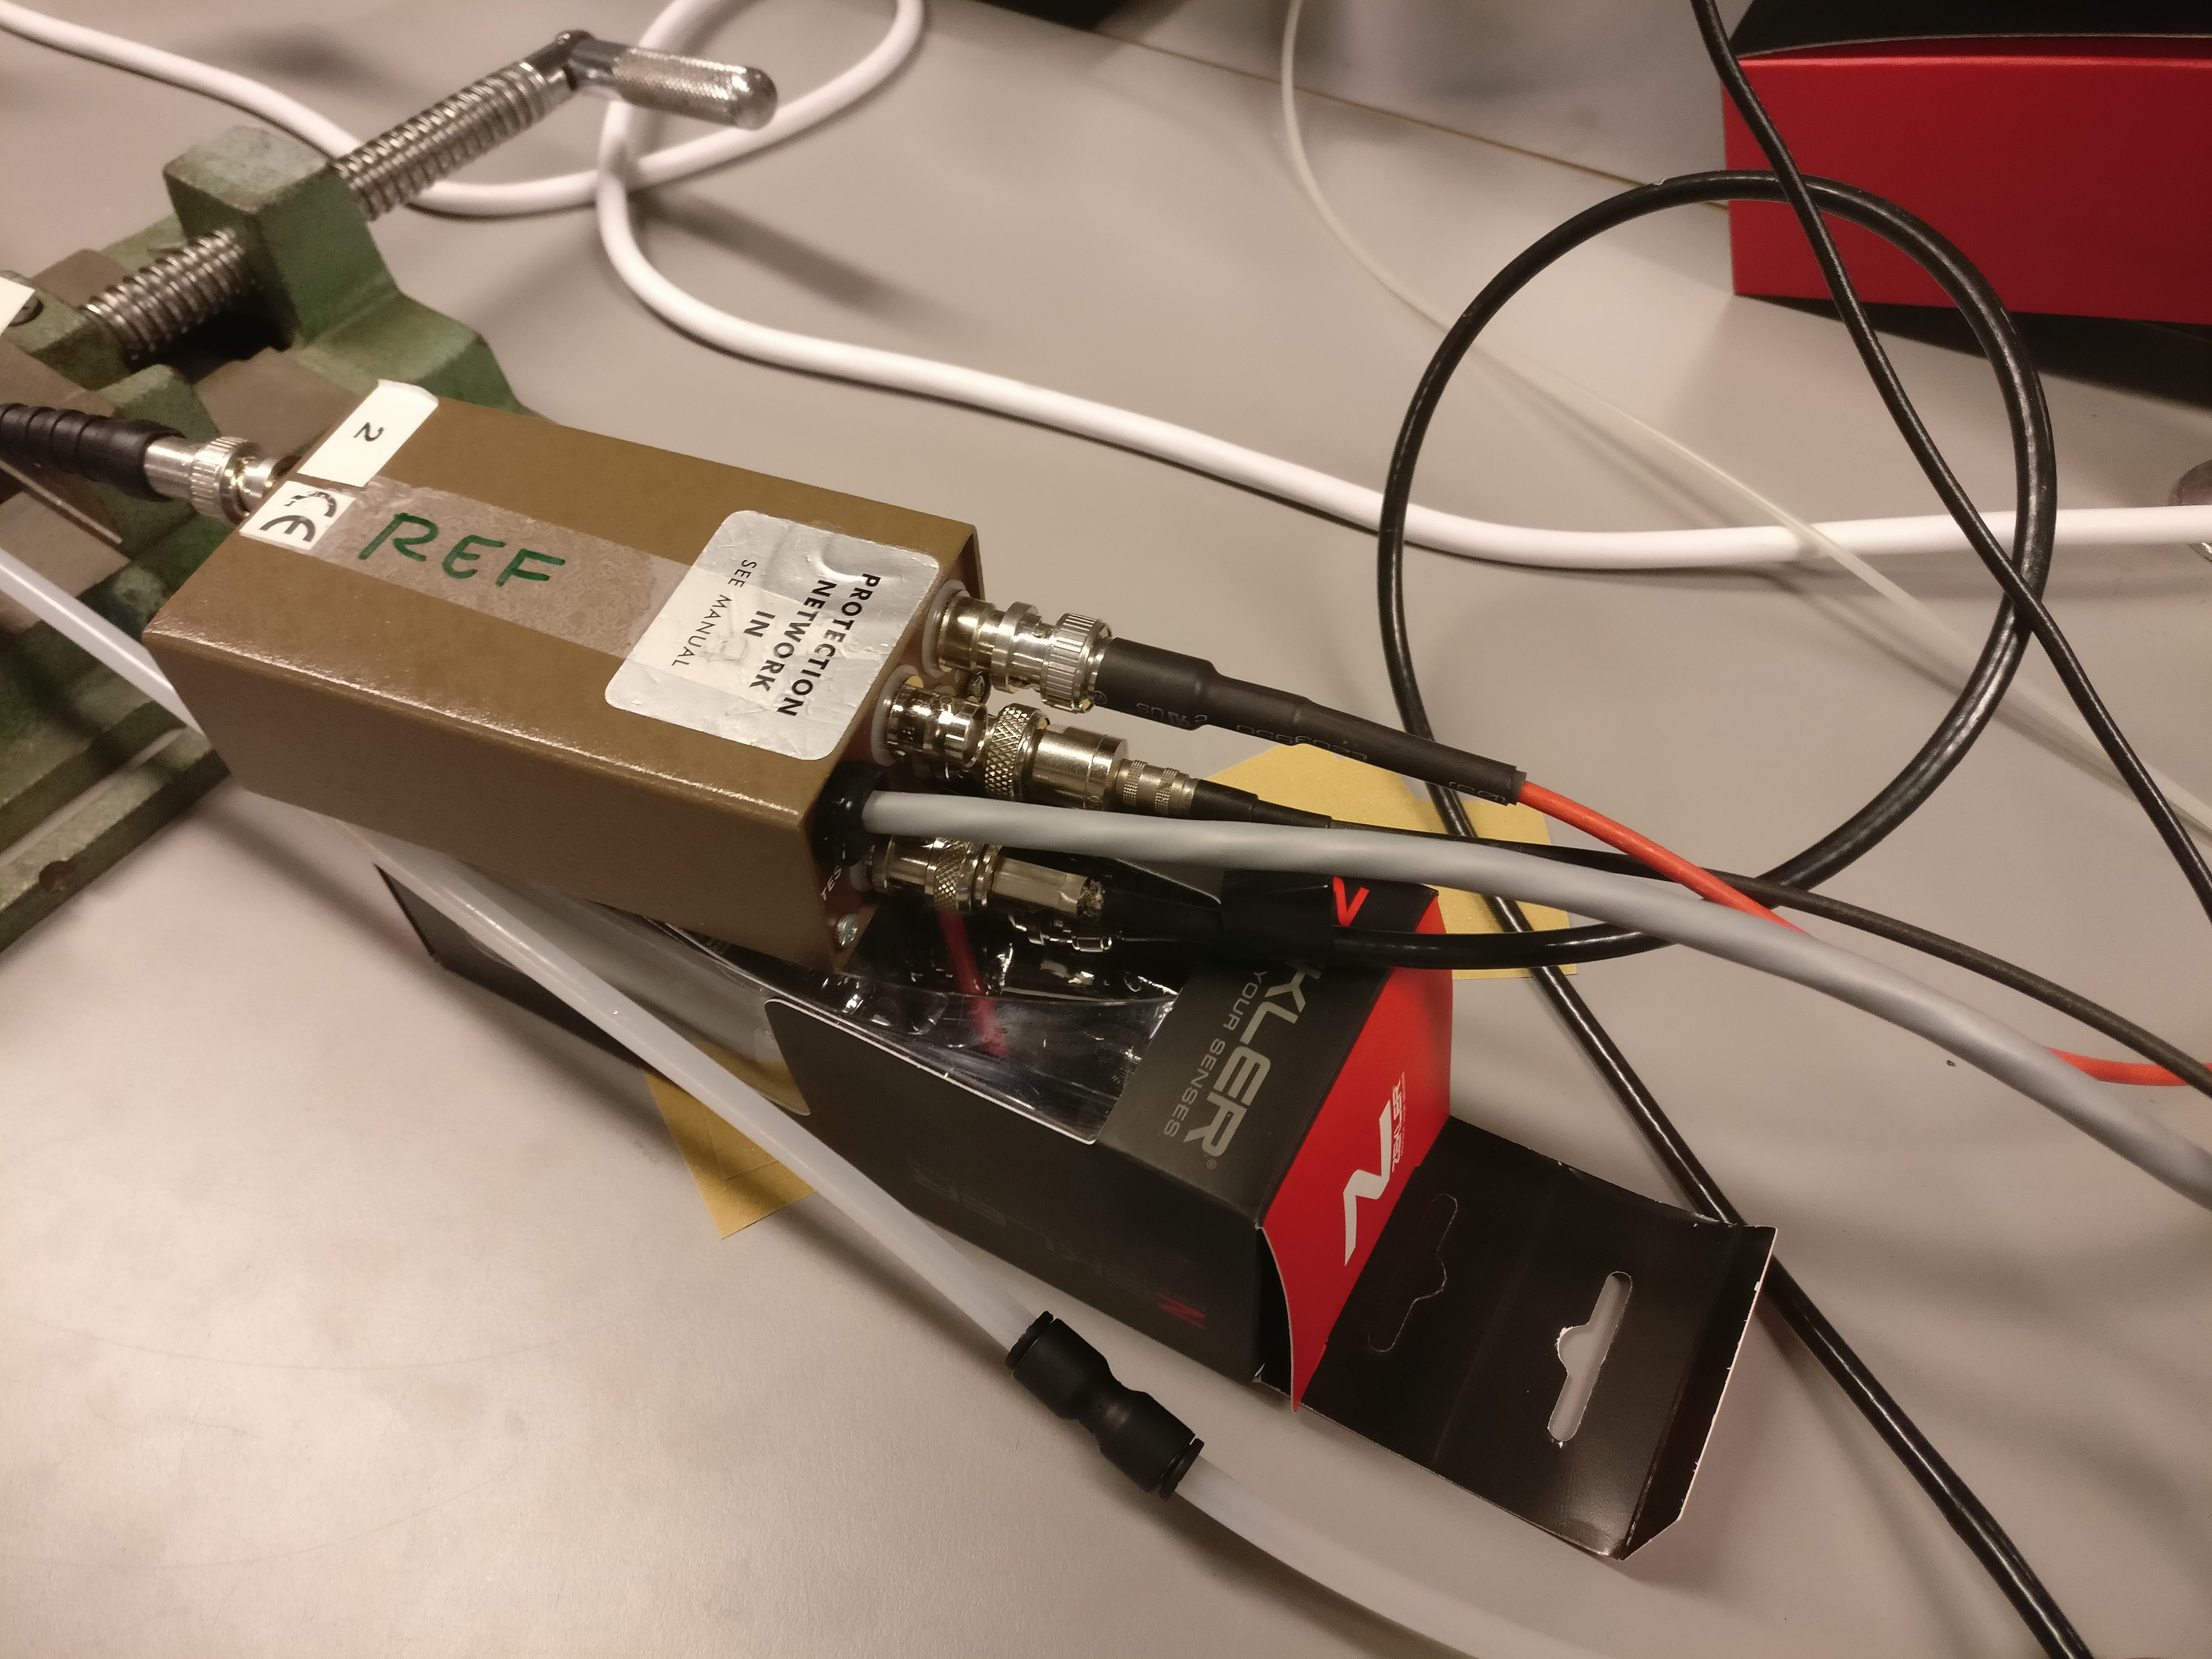
\includegraphics[width=\textwidth]{graphics/preamplifier.jpg}
    \caption{}
    \label{fig:preamp_photo}
  \end{subfigure}
  ~
  \begin{subfigure}[b]{0.5\textwidth}
    \includegraphics[width=\textwidth]{graphics/amplifier_photo.jpg}
    \caption{}
    \label{fig:ampli_gene}
  \end{subfigure}
  \caption{a) Photograph of the preamplifier unit. b) Photograph of the pulse generator used to inject pulses into the preamplifer, and the coarse gain amplifier used in front of the MCA.}
\end{figure}

Both system contribute to increase the overall number of signal electrons collected per avalanche occuring in the drift chamber. The overall gain in signal, between the drift chamber electrode and the final Multi-Channel Analyzer (MCA) reading out data, is given by equation \ref{eq:gain_system}.

\begin{equation}
  \label{eq:gain_system}
  Q_{MCA} = Q_{drift}\cdot G_{pre}\cdot G_{coarse}
\end{equation}


\subsection{Calibration of the pre-amplifier gain}
 Calibrated pulses of various intensities were injected into the electronics, and the output was displayed onto an oscilloscope to evaluate the gain of the preamplifier, $G_{pre}$ and its uncertainty. Figure \ref{fig:preamp_gain} shows the result of this measurements, where the data was fitted to a line. Note that the slope of the line corresponds to 10 times the gain of the preamplifier: this is because the entire calibration measurement was performed at a nominal coarse gain of 10. This correction factor is accounted for when quoting the gain that is only due to the pre-amplifier, $G_{pre} = 6.41 \pm 0.01$.

\begin{figure}[H]
  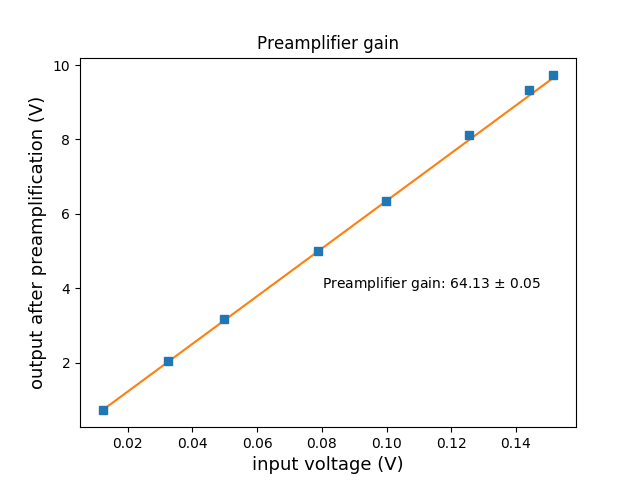
\includegraphics[scale=0.5,width=0.5\textwidth]{graphics/preamp_gain_calibration.png}
  \caption{Output voltage of pulses injected into the pre-amplifier electronics. The quoted gain on the figure and the slope of the line differ by a factor of 10.}
  \label{fig:preamp_gain}
\end{figure}

In later sections of this report, it will be more useful to quote the preamplifier gain in units of $d.c/V$, as the later measurements have been done using the Multichannel analyzer (MCA), and not of the oscilloscope. Figure \ref{fig:preamp_gain_mca} presents the preamplifier gain in these units. Once again, a correction factor of 10 is applied to remove the coarse gain value from the result.

\begin{figure}[H]
  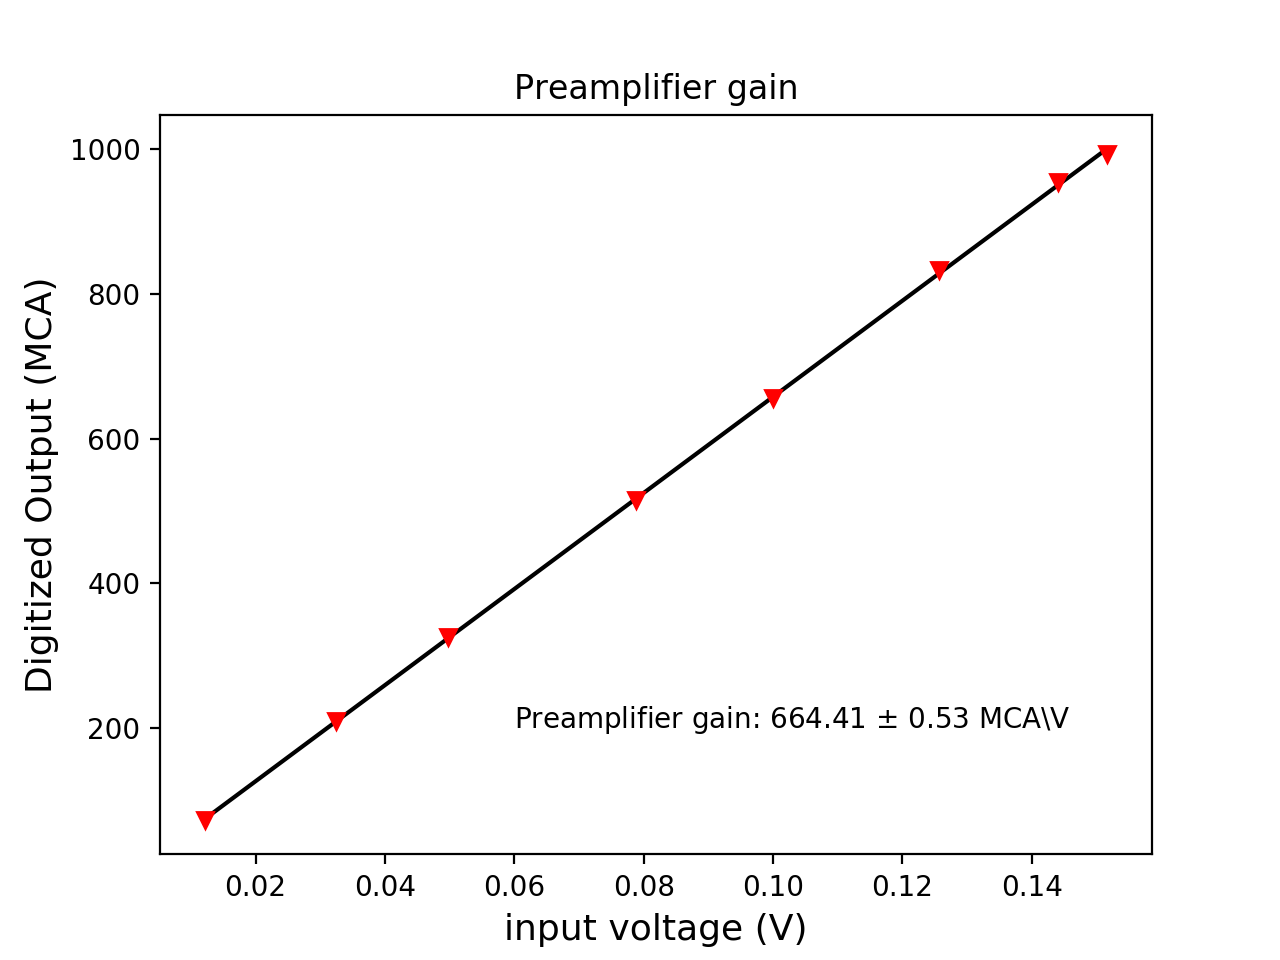
\includegraphics[scale=0.5,width=0.5\textwidth]{graphics/preamp_gain_calibration_plus_conversionfactor.png}
  \caption{Measurement of the preamplifier gain, in terms of digital counts taken from the MultiChannel Analyzer (MCA) The quoted gain on the figure and the slope of the line differ by a factor of 10.}
  \label{fig:preamp_gain_mca}
\end{figure}


\subsection{Calibration of the Coarse Gain amplifier}
\label{sec:coarse}
To estimate the uncertainty on the coarse gain amplifier, subsequent runs of Fe$^{55}$ and Am$^{241}$ spectra acquisitions were made at the same operating voltage, but different coarse gain settings. These measurements allowed us to measure the \textit{ratios of coarse gains} between subsequent settings of the amplifier knob, with corresponding uncertainties.

Figure \ref{fig:coarse_gain} shows the result of this analysis. Since the data acquired only allowed us to measured ratios of gain settings, the uncertainties of the absolute amplifier gain are simply assumed to scale with the default setting of 10, used in the previous calibration measurement. This means that for the purpose of error propagation, each coarse gain was defined with respect to the following rules

$$
G_{coarse} = \left\{
\begin{array}{ll} 
  10\cdot\Pi_{j>i}^{j\leq10}\frac{G_{j}}{G_{i}} & (i) \in [2,4] \\
  10 & i=10 \\
  10\cdot\Pi_{j>i}^{j\leq 100}\frac{G_{j}}{G_{i}} & i \in [20,40] 
\end{array}
\right.
$$

where $j$ is the higher level of a pair of coarse gain settings. Figure \ref{fig:coarse_gain} presents the various ratios of gain settings measured, using both the Fe$^{55}$ and Am$^{241}$ source. The red data point show the result of combining both results, which allows us to get better estimates of the gain ratio uncertainties.

\begin{figure}[H]
  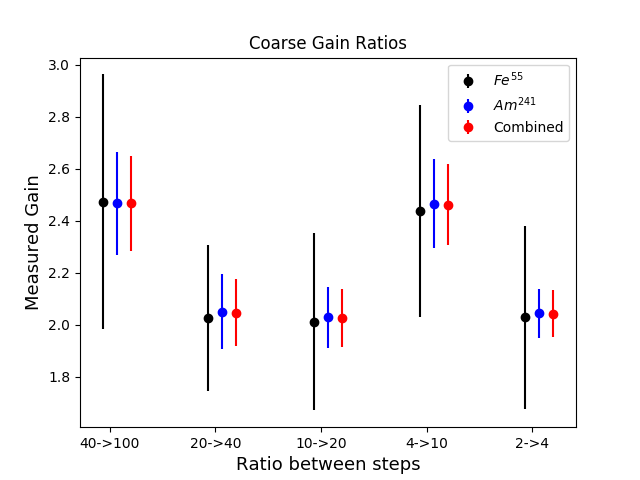
\includegraphics[width=0.5\textwidth]{graphics/coarse_gain_calibration.png}
  \caption{Determination of the coarse gain amplification uncertainties. Results are presented in the form of gain ratios between every adjacent setting of the coarse gain knob. The combined value and uncertainty on each measurement is shown by the red data points.}
  \label{fig:coarse_gain}
\end{figure}


As stated above, the use of gain ratio is useful for propagating the uncertainty on $G_{coarse}$, when considering the effect of systematics on the global yield of charge carrier in the drift chamber (see section \ref{sec:systematics}).
